%%% License: Creative Commons Attribution Share Alike 4.0 (see https://creativecommons.org/licenses/by-sa/4.0/)
%%% Slides are based heavily on earlier versions of this course taught by Jesper Rudiger.

\documentclass[english,10pt
%,handout
,aspectratio=169
]{beamer}
%%% License: Creative Commons Attribution Share Alike 4.0 (see https://creativecommons.org/licenses/by-sa/4.0/)
%%% Slides are based heavily on earlier versions of this course taught by Jesper Rudiger and Peter Norman Sorensen.

\DeclareGraphicsExtensions{.eps, .pdf,.png,.jpg,.mps,}
\usetheme{reMedian}
\usepackage{parskip}
\makeatother

\renewcommand{\baselinestretch}{1.1} 

\usepackage{amsmath, amssymb, amsfonts, amsthm}
\usepackage{enumerate}
\usepackage{hyperref}
\usepackage{url}
\usepackage{bbm}
\usepackage{color}

\usepackage{tikz}
\usepackage{tikzscale}
\newcommand*\circled[1]{\tikz[baseline=(char.base)]{
		\node[shape=circle,draw, inner sep=-20pt] (char) {#1};}}
\usetikzlibrary{automata,positioning}
\usetikzlibrary{decorations.pathreplacing}
\usepackage{pgfplots}
\usepgfplotslibrary{fillbetween}
\usepackage{graphicx}

\usepackage{setspace}
%\thinmuskip=1mu
%\medmuskip=1mu 
%\thickmuskip=1mu 


\usecolortheme{default}
\usepackage{verbatim}
\usepackage[normalem]{ulem}

\usepackage{apptools}
\AtAppendix{
	\setbeamertemplate{frame numbering}[none]
}
\usepackage{natbib}




\title{Financial Markets Microstructure \\ Lecture 10}

\subtitle{Limit order book, part 1\\
	Chapter 6.1-6.2 of FPR}

\author{Egor Starkov}

\date{K{\o}benhavns Unversitet \\
	Spring 2022}




\begin{document}
\AtBeginSection[]{
\frame<beamer>{
\frametitle{This lecture:}
\tableofcontents[currentsection,currentsubsection]
}}
\frame[plain]{\titlepage}

%\section{Revision and readings}

\begin{frame}{Last time}
	\begin{itemize}
		\item The Kyle model helps us analyze market depth:
		\begin{itemize}
			\item Hence, it tells us something about how adverse selection causes spread to vary with trade size
			\item The model has batch clearing instead of the single-unit market of GM
		\end{itemize}
		\item We can use insights from theory to estimate the importance of different components of the spread
		\begin{itemize}
			\item Perhaps surprisingly, order costs are by far the largest cost (but estimated on major stocks)
			\item Around 19\% of trading is informed
			\item Adverse selection is stronger for less liquid/small-cap stocks
		\end{itemize}
	\end{itemize}
\end{frame}


\begin{frame}{Homework}
	\begin{itemize}
		\item Read the Economist article on the corporate bond market. 
		\\
		Discuss the following questions:
		\begin{enumerate}
			\item How does corporate bond market liquidity differ from the stock market liquidity? Why?
			\item Why do investors' liquidity expectations matter?
			\item How do investors form their expectations of liquidity?
			\item Can we \emph{measure investors' expectations} of liquidity?
		\end{enumerate}
	\end{itemize}
\end{frame}


%\begin{frame}{Exercise}
%	% the conclusions from last time may lead us into thinking that informed trading is no big deal. These articles aim to argue the converse
%	\begin{itemize}
%		\item I uploaded two articles from the Economist, March 7, 2014, both on potential manipulation of prices
%		\item Consider these two issues:
%		\begin{itemize}
%			\item What motivates a trader to manipulate an asset's price? 
%			\item Is manipulation easier in a very liquid or a very illiquid market?
%			% less liquid requires less effort to manipulate the price, but it looks less credible
%		\end{itemize}
%	\end{itemize}
%\end{frame}



\section{LOB Markets: Introduction}

\begin{frame}<handout:0>{Introduction}
	\begin{itemize}
		\item There's a reason that first models of financial markets (GM and Kyle) explored dealer markets...
	\end{itemize}
\end{frame}


\begin{frame}<handout:0>
	\centering
	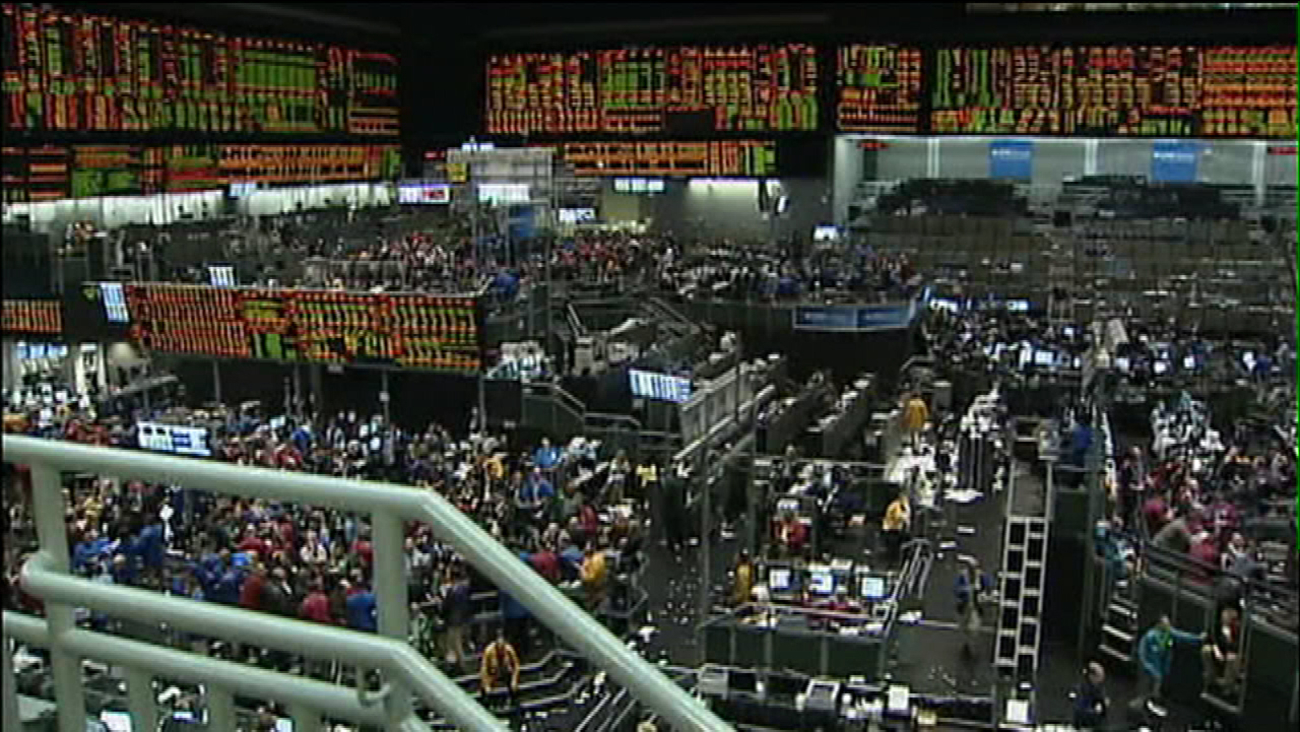
\includegraphics[scale=0.5]{pics/mkt20}
	
	Financial market in 1985
\end{frame}


\begin{frame}<handout:0>
	\centering
	
\includegraphics[scale=0.19]{pics/mkt21}
	
	Financial market today
\end{frame}


\begin{frame}{LOB Markets: Liquidity Demand}
	\begin{itemize}
		\item Most markets are order-driven these days
		\begin{itemize}
			\item Some exchanges combine LOBs and dealers
		\end{itemize}
		\item There is also conceptual convenience in starting with dealer models...
		\item ``Dealer'' is an abstraction of the ``market'':
		\begin{center}
			\structure{Trader interacting with the dealer} $\approx$ \alert{Trader interacting with the market}
		\end{center}
		So for a \textbf{liquidity demander} who submits market orders, it does not really matter who to trade against.
	\end{itemize}
\end{frame}


\begin{frame}{LOB Markets: Liquidity Providers}
	But \alert{liquidity provision} works quite differently in LOB markets:
	\begin{enumerate}
		\item Traders have a choice between \structure{demanding and supplying liquidity} (market vs limit orders) -- so LO should be no worse than MO for trading
		\item LO give better prices but suffer from execution risk
		\item Conditional on electing to trade via LO, traders face a \structure{different informational environment} than the dealer
		\item Also there's discriminatory pricing: LO execute each at their posted price, while a dealer can clear everything at uniform price.
	\end{enumerate}
	We look at the two latter issues today; two former next time.
\end{frame}


\begin{frame}{LOB Markets: Modelling Issues}
	A limit order is $(t,x,p)$: submission time $t$, quantity $x$, price $p$.
	
	Modelling LOBs properly is very difficult, many factors to account for:
	\begin{enumerate}
		\item Traders' \structure{action set} is large: submit buy/sell LO/MO, how much, choose price if LO
		\item \structure{Dynamics} is relevant: choose when to submit, when to cancel/resubmit (since LO might not execute)
		\item \structure{State} of LOB is rich: trader's choice depends on other LOs in the book (though not all of them might be observable)
		\item Private information affects not just valuation, but \structure{expectations} about LOB evolution...
	\end{enumerate}
	So we'll look at very simple models that explore different slices of this problem.
\end{frame}


%\begin{frame}{Introduction}
%	\begin{itemize}
%		\item \structure{Price discrimination}:  LOB has discriminatory pricing of larger orders
%		\begin{itemize}
%			\item Difference to Kyle's (auction) model: in LOB, total order size is not observed, you only know that your limit order has been `hit'
%			\item \cite{glosten_is_1994} provides a Glosten-Milgrom style model of the price schedule offered (i.e., how much volume supplied at the limit prices)
%		\end{itemize}
%		\item \structure{Ticks}: Often prices are discrete and must lie at a tick (e.g. at NYSE, ticks are multiples of 1 cent) --  tick size is the increment btw prices:
%		\begin{itemize}
%			\item Prioritized limit orders become profitable when there are ticks 
%			(since no `marginal undercutting')
%			\item We will analyze the effects of changing ticks, priority rules
%		\end{itemize}
%		\item \structure{Interpretation}: One way of thinking of an LOB is that dealers post limit orders, as in the GM model
%	\end{itemize}
%\end{frame}



\section{Static Analysis: Glosten Model (continuous)}

\begin{frame}{\cite{glosten_is_1994} model}
	\begin{itemize}
		\item Begin by looking at \cite{glosten_is_1994} model
		\begin{itemize}
			\item (Probably) the first model of LOB markets
			\item Does not capture all of traders' choices
			\item Consider it to be ``one step towards LOB markets from Kyle model''.
		\end{itemize}
		\item Questions simple:
		\begin{itemize}
			\item What drives the prices? Are they efficient?
			\item How are prices different from dealer markets?
			\item How is LOB depth determined?
		\end{itemize}
	\end{itemize}
\end{frame}


\begin{frame}{Continuous model: Limit order book}
\begin{itemize}
	\item \textbf{Single asset}: Unknown value $v$ with cumulative distribution  $G(v)$
	\item \textbf{Limit order book} (composed by competitive limit traders): 
	\begin{itemize}
		\item Focus on the ask side of the market (limit orders to sell vs market order to buy)
		\item Prices vary with volume $q$. Posted limit orders: $P'(q)$
		\item A market buy order of size $q$ will `walk up the book' until the final bit of it is cleared at price $P'(q)$
		\item The entire payment for buying volume $q$ is then
		\[
		P(q) = \int_0^q P'(\tilde{q}) \, d\tilde{q}.
		\]
		\item The average price is 
		\[
		p(q) = \frac{P(q)}{q}.
		\]
	\end{itemize}
	\pause
	\item Sanity check: in the Kyle model, did the dealer announce \alert{marginal ($P'(q)$)} or \structure{average ($p(q)$)} price schedule?
\end{itemize}
\end{frame}


\begin{frame}{Continuous model: Marginal rate of substitution}
	\begin{columns}
		\begin{column}{0.7\linewidth}
			\begin{itemize}
				\item \textbf{Single market trader} $i$ per period (as in GM/Kyle)
				\item $\theta_i(q)$ is trader $i$'s marginal rate of substitution (marginal valuation for $q$th unit of the asset)
				\item If an incoming trader $i$ chooses a market buy order $q$ and parts with cash $P(q)$, we should have: \[\theta_i(q) = P'(q).\]
				\item Assume $\mathbb{E}[v|\theta_i(q) = \theta]$ is strictly increasing in $\theta$
				\begin{itemize}
					\item If incoming traders are to some extent informed, it's reasonable to suppose that for a given $q$, higher $\theta_i(q)$ indicates higher $v$
					\item In the Kyle model we derived it, here we'll just assume that this holds.
				\end{itemize}
			\end{itemize}
		\end{column}
		\begin{column}{0.3\linewidth}
			\includegraphics[scale=0.2]{pics/glosten1}
			\vspace{3em}
		\end{column}
	\end{columns}
\end{frame}


\begin{frame}{Continuous model: Market makers}
	\begin{itemize}	
		\item \textbf{Limit traders} are competitive, post limit orders
		\item Limit price $P'(q)$ quoted for the $q$-th unit is relevant only if the trader places a market order of $q$ or larger, i.e. $\theta_i(q) \geq P'(q)$
		\item Hence, if supply is competitive then
		\[
		\structure{P'(q) = \mathbb{E}[v|\theta_i(q) \geq P'(q)]}
		\]
		%\item Notice that all we know if limit price $P'(q)$ is `hit' is that the trader's marginal valuation was \textit{at least} $P'(q)$
	\end{itemize}
\end{frame}


\begin{frame}{Continuous model: Equilibrium}
	The assumed correlation of $v$ and $q$ implies that
	\begin{align}
	P'(q) = \mathbb{E}[v|\theta_i(q) \geq P'(q)] > \mathbb{E}[v|\theta_i(q) = P'(q)]
	\end{align}
	\pause
	\begin{block}{Implications}
		\begin{itemize}
			\item Thus, market makers (ex post) profit on the sale of the last units
			\item At small realized trades, $q \simeq 0$, MM always profit
			\item Even with continuous prices, there is a non-zero \structure{inside spread} between ask and bid prices as the order size goes to zero (contrast with Kyle)
			% The reason is that in the limit order market, liquidity suppliers cannot make their quotes contingent on the total size of market orders. As a result, the limit orders at the top of the book are more exposed to adverse selection.
			\item After a trade of size $q$, new expected asset value is below $P'(q)$. \pause 
			
			\structure{New expected value = $\mathbb{E}[v|\theta_i(q)=P'(q)]<\mathbb{E}[v|\theta_i(q) \ge P'(q)]=P'(q)$}. Often new limit orders will be posted below $P'(q)$ -- price reversal.
		\end{itemize}
	\end{block}
\end{frame}


%\section{Static Analysis: Glosten Model (discrete ticks)}
%
%\begin{frame}{Intermission}
%	\begin{itemize}
%		\item The general model above outlines some basic differences between LOB and dealer markets
%		\begin{itemize}
%			\item Adverse selection affects prices differently
%		\end{itemize}
%		\item It neglects the \structure{discreteness of prices}:
%		\begin{itemize}
%			\item Often prices are discrete and must lie at a tick --  tick size is the increment b/w prices
%			\item E.g. at NYSE it was \$1/8 for stocks with prices over one dollar until June 1997, when, under regulatory pressure, it was reduced to \$1/16 and finally, in 2000, to one cent.
%			\item Prioritized limit orders become profitable when there are ticks (since no `marginal undercutting')
%		\end{itemize}
%	\end{itemize}
%\end{frame}
%
%
%\begin{frame}{Discrete model: Setup}
%	\begin{itemize}
%		\item \textbf{Asset}: Continue with single asset with value $v \sim G$
%		\item \textbf{Market order $q$} correlated with $v$
%		\begin{itemize}
%			\item Unconditional c.d.f. $F(q)$
%			\item Again, focus on the ask side of the book, $q>0$
%		\end{itemize}
%		\item \textbf{Discrete price grid}
%		\begin{itemize}
%			\item $A_1$ is lowest price tick above $\mu$
%			\item $A_k-A_{k-1}>0$ is the tick size
%		\end{itemize}
%		\item \textbf{Limit orders}
%		\begin{itemize}
%			\item \textit{Time prioritized}: first posted, first executed
%			\item \textit{Display cost}: $C$ per unit (paid regardless of whether order executes)
%			% This display cost is here for the model to work even without adverse selection
%			\item Let $y_k$ denote the amount supplied at price $A_k$
%			\item Let $Y_k=\sum_{j=1}^k y_j$ be cumulative volume (depth) supplied at or below $A_k$
%			% Y_k(A_k) is the inverse of P(q)
%		\end{itemize}
%	\end{itemize}
%\end{frame}
%
%
%\begin{frame}{Discrete model: Equilibrium}
%	%Let $\mathbb{E}[v|q \geq Y_k]=\mathbb{E}[v|\theta_i(q) \geq P'(q)]$.
%	Let $\mathbb{E}[v|q \geq Y_k]=\mathbb{E}[v|\theta_i(q) \geq A_k]$.
%	\begin{itemize}
%		\item \textbf{Competition}: Limit orders are supplied at each tick until the \structure{last order earns zero profit}
%		\item \textbf{Zero-profit condition}:
%		\[
%		\mathbb{P}(q \geq Y_k)[A_k-\mathbb{E}[v|q \geq Y_k]] - C = 0,
%		\]
%		solved by
%		\begin{block}{}
%			\[
%			A_k = \underbrace{\mathbb{E}[v| q \geq Y_k]}_{\text{\alert{Adverse selection}}} + \underbrace{\frac{C}{\mathbb{P}(q\geq Y_k)}}_{\text{\alert{Execution risk}}}
%			\]
%		\end{block}
%		(\textbf{NOTE}: \structure{we actually need to solve for $Y_k$ given $A_k$})
%		%\item \textbf{Adverse selection}: Captured by  $\mathbb{E}[v| q \geq Y_k] $
%		%\begin{itemize}
%		%	\item Unlike most of what we had before, this model works even without adverse selection
%		%\end{itemize}
%	\end{itemize}
%\end{frame}


\begin{frame}{Conclusion}
	\begin{itemize}
		\item First look into LOB markets using \cite{glosten_is_1994}.
		\item Limit traders act in the same capacity as the dealer did before
		\begin{itemize}
			\item but face different \alert{informational environment}
			\item so act differently
			\item which leads to different market outcomes
		\end{itemize}
		\item With discrete ticks and time priority, even competitive limit traders can get positive profit
	\end{itemize}
\end{frame}


\begin{frame}{Next time}
	\begin{itemize}
		\item What happens if we restrict prices to discrete ticks?
		\item Many aspects of market design (tick size, priority rules) are all double-edged swords, swing them carefully
		%\item Dynamic analysis: traders can choose between limit and market orders
	\end{itemize}
\end{frame}


%\begin{frame}{Homework}
%	\begin{itemize}
%		\item Thinking in the framework of the discrete model: suppose tick size is actually zero; quotes can be placed in a continuous price space. Suppose that there is price priority. What then is the role of time priority, so that first-come quotes at identical prices are served first?
%		\item If you could choose between trading at discriminatory prices in a limit order book, or to reveal your order size to a dealer, what would influence your choice?
%		% ex1 is on informed trading
%		% ex5 is on make-or-take choice 
%		\item Solve exercise 1 on pages 232-233 (ch.6) in the textbook. Note that you need to use Bayes' rule to assess the conditional distribution over $v$ given a market order of size $q$
%		%\item Solve exercise 5 on page 235 in the textbook on the effect of fees charged for limit orders and market orders
%	\end{itemize}
%\end{frame}





\appendix
\begin{frame}<handout:0>[allowframebreaks]{References}
	\bibliography{../teaching}
	\bibliographystyle{abbrvnat}
\end{frame}




\end{document} 